\documentclass[a5paper, 8pt]{extarticle}
\usepackage[T2A]{fontenc}
\usepackage[utf8]{inputenc}
\usepackage[russian]{babel}
\usepackage[left=1.5cm,right=1.5cm,top=1.5cm,bottom=1.5cm]{geometry} 

\usepackage{amsmath}
\usepackage{amsfonts}
\usepackage{amssymb}
\usepackage{graphicx}
\usepackage{tabularx}
\usepackage{indentfirst}

%Колонтитулы
\usepackage{lastpage} 
\usepackage{fancybox,fancyhdr}
\fancyhead[R]{Справочник формул по математике}
\fancyhead[L]{Владимир Анатольевич Калитвин}
\fancyhead[C]{}
\fancyfoot[R]{Калитвин В.А. (kalitvin@gmail.com)}
\fancyfoot[L]{Страница \thepage \; из \pageref{LastPage}}
\fancyfoot[C]{}
\pagestyle{fancy}
%

%Рамки
\usepackage{framed}
%

%Color
\usepackage{color,colortbl}
\definecolor{Gray}{gray}{0.9}

%Graphicx path
\graphicspath{ {img/} }

%Точки в заголовках
\renewcommand{\thesection}{\arabic{section}.}
\renewcommand{\thesubsection}{\arabic{section}.\arabic{subsection}.}

\begin{document}
\author{Калитвин В.А.\\
kalitvin@gmail.com}
\title{Справочник формул по математике}
\maketitle
\thispagestyle{empty}
\newpage

\section{Признаки делимости}

\textbf{на 2} --- последняя цифра числа чётная

\textbf{на 3} --- сумма цифр числа делится на 3

\textbf{на 4} --- две последние цифры числа нули или образуют число, делящиеся на 4

\textbf{на 5} --- последняя цифра числа 0 или 5

\textbf{на 6} --- число должно делится на 2 и на 3

\textbf{на 8} --- три последние цифры числа нули или образуют число, делящееся на 8

\textbf{на 9} --- сумма цифр числа делится на 9

\textbf{на 11} --- сумма цифр, стоящих на четных местах, отличается от суммы цифр, стоящих на нечётных местах, на число, кратное 11

\textbf{на 25} --- две последние цифры цисла 00, 25, 50 или 75


\section{Формулы сокращенного умножения}

Квадрат суммы
$$ (a+b)^2=a^2+2ab+b^2$$

$$ (a+b+c)^2=a^2+b^2+c^2+2ab+2bc+2ac$$

Квадрат разности
$$(a-b)^2=a^2-2ab+b^2$$

Разность квадратов
$$a^2-b^2=(a-b)(a+b)$$

Куб суммы
$$(a+b)^3=a^3+3a^2b+3ab^2+b^3$$

Куб разности
$$(a-b)^3=a^3-3a^2b+3ab^2-b^3$$

Сумма кубов
$$a^3+b^3=(a+b)(a^2-ab+b^2)$$

Разность кубов
$$a^3-b^3=(a-b)(a^2+ab+b^2)$$

Для $n\in N$
$$a^n-b^n=(a-b)(a^{n-1}+a^{n-2}b+a^{n-3}b^2+\dots +ab^{n-2}+b^{n-1})$$

Если $n$ - четное
$$a^n-b^n=(a+b)(a^{n-1}-a^{n-2}b+a^{n-3}b^2-\dots +ab^{n-2}+b^{n-1})$$

Если $n$ - нечетное
$$a^n+b^n=(a+b)(a^{n-1}-a^{n-2}b+a^{n-3}b^2-\dots -ab^{n-2}+b^{n-1})$$

Бином Ньютона
$$(a+b)^n=\sum\limits_{k=0}^n C_n^ka^{n-k}b^k=$$
$$=C_n^0a^n+C_n^1a^{n-1}b^1+C_n^2a^{n-2}b^2+\dots +C_n^{n-1}a^1b^{n-1}+C_n^nb^n,$$
где $C_n^k=\frac{n!}{k!(n-k)!}$ --- число сочетаний из $n$ по $k.$

\section{Свойства степени}

$$
\begin{array}{ll}
a^0=1  & a^m\cdot a^n=a^{m+n}\\
a^m: a^n=a^{m-n} & a^{-n}=\frac{1}{a^n}\\
(a^m)^n=a^{mn} & (\frac{a}{b})^{-m}=(\frac{b}{a})^{m}\\
(a\cdot b)^m=a^m\cdot b^m & a^{\frac{1}{n}}=\root{n}\of{a}\\
(\frac{a}{b})^m =\frac{a^m}{b^m} & a^{\frac{m}{n}}=\root{n}\of{a^m}\\
\end{array}
$$

\section{Свойста квадратного (арифметического) корня}

$$
\begin{array}{ll}
\sqrt{a}\cdot \sqrt{b} = \sqrt{ab}  & \root{n}\of{a}=\root{nk}\of{a^k} \\
\frac{\sqrt{a}}{\sqrt{b}}=\sqrt{\frac{a}{b}}, b\not= 0 & \root{n}\of{a}\cdot \root{n}\of{b}=\root{n}\of{a\cdot b}\\
(\sqrt{a})^m=\sqrt{a^m} & \frac{\root{n}\of{a}}{\root{n}\of{b}}=\root{n}\of{\frac{a}{b}}, b\not=0\\
\sqrt{ab}=\sqrt{|a|}\cdot \sqrt{|b|} & (\root{n}\of{a})^m = \root{n}\of{a^m}\\
\sqrt{\frac{a}{b}}=\frac{\sqrt{|a|}}{|b|}, b\not=0 & \root{n}\of{\root{m}\of{a}} = \root{nm}\of{a}\\
\sqrt{a^m}=(\sqrt{|a|})^m
\end{array}
$$

\section{Модуль числа}

$$|a|=\left\{
\begin{array}{l}
a, a\ge 0,\\
-a, a<0,
\end{array}
\right., 
|a|=\sqrt{a^2}
$$

Свойства
$$ 
\begin{array}{lll}
|a|\ge 0; \ \ \ \ \ & |a\cdot b|=|a|\cdot |b| \ \ \ \ & |a+b|\le |a|+|b|\\
|a|=0 \Leftrightarrow a=0 & \left| \frac{a}{b}\right|=\frac{|a|}{|b|}, b\not=0& |a-b|\ge ||a|-|b|| 
\end{array}
$$

Геометрический смысл модуля

$|a|$ --- расстояние от $0$ до точки $a.$

$|a-b|$ --- расстояние между точками $a$ и $b$.

\section{Прогрессии}

\textbf{Арифметическая прогрессия}
$$
a_{n+1}=a_n+d,$$ 

где $d$ --- разность  прогрессии

Формулы $n$-го члена
$$a_n=a_1+(n-1)d$$
$$a_n=a_k+(n-k)d$$
$$a_n=\frac{a_{n-k}+a_{n+k}}{2}$$

Формулы суммы первых $n$ членов
$$S_n=\frac{2a_1+(n-1)d}{2}\cdot n=\frac{a_1+a_n}{2}\cdot n$$

Формула для разности
$$d=a_{n+1}-a_n$$

Если $n+m=k+p,$ то
$$a_n+a_m=a_k+a_p$$

Сумма последовательных натуральных чисел от  1 до $n:$
$$S=\frac{n(n+1)}{2}$$

\textbf{Геометрическая прогрессия}
$$
b_{n+1}=b_n\cdot q,$$ 

где $q\not= 0$ --- знаменатель  прогрессии

Формулы $n$-го члена
$$b_n=b_1\cdot q^{n-1}$$
$$b_n=b_k\cdot q^{n-k}$$
$$b_n^2=b_{n-k}\cdot b_{n+k}$$

Формулы суммы первых $n$ членов
$$S_n=b_1\frac{1-q^n}{1-q}=b_1\frac{q_n-1}{q-1}, q\not=1$$
$$S_n=b_1\cdot n, q=1$$

Формула для знаменателя
$$q=\frac{b_{n+1}}{b_n}$$

Если $n+m=k+p,$ то
$$b_n\cdot b_m=b_k\cdot b_p$$

Сумма бесконечно убывающей геометрической прогрессии
$$S=\frac{b_1}{1-q}, |q|<1$$

\section{Тригонометрия}

\textbf{Знаки тригонометрических функций по четвертям}

\begin{center}
\begin{tabular}{ccc}
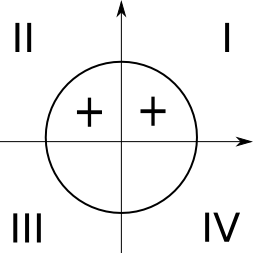
\includegraphics[width=0.25\linewidth]{img01.png} \ & 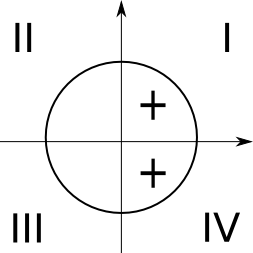
\includegraphics[width=0.25\linewidth]{img02.png} \ & 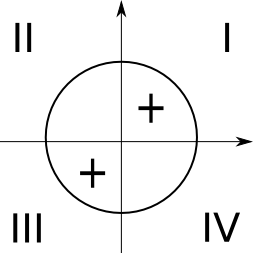
\includegraphics[width=0.25\linewidth]{img03.png} \ \\ 
$\sin x$ & $\cos x$ & $\tg x, \ctg x$ \\ 
\end{tabular} 
\end{center}

\textbf{Тригонометрические тождества}

$$\sin^2\alpha+\cos^2\alpha=1$$

$$\tg\alpha =\frac{\sin\alpha}{\cos\alpha}$$

$$\ctg\alpha =\frac{\cos\alpha}{\sin\alpha}$$

$$\tg\alpha \cdot \ctg\alpha = 1$$

$$|\cos \alpha |=\sqrt{1-\sin^2\alpha}$$

$$|\sin \alpha |=\sqrt{1-\cos^2\alpha}$$

$$\tg\alpha = \frac{1}{\ctg\alpha}$$

$$\ctg\alpha = \frac{1}{\tg\alpha}$$

$$1+\tg^2\alpha =\frac{1}{\cos^2\alpha}=sec^2\alpha$$

$$1+\ctg^2\alpha =\frac{1}{\sin^2\alpha}=cosec^2\alpha$$

\textbf{Формулы сложения тригонометрических функций}

$$\sin(\alpha \pm \beta )=\sin \alpha \cos \beta \pm \cos \alpha \sin \beta $$

$$\cos(\alpha \pm \beta )=\cos \alpha \cos\beta \mp \sin\alpha\sin\beta$$

$$\tg(\alpha\pm\beta)=\frac{\tg\alpha\pm\tg\beta}{1\mp\tg\alpha\tg\beta}$$

$$\ctg(\alpha\pm\beta)=\frac{\ctg\alpha\ctg\beta\mp1}{\ctg\beta\pm\ctg\alpha}$$

\textbf{Тригонометрические функции двойного аргумента}

$$\sin2\alpha=2\sin\alpha\cos\alpha$$
$$\cos2\alpha=\cos^2\alpha-\sin^2\alpha=1-2\sin^2\alpha=2\cos^2\alpha-1$$
$$\tg2\alpha=\frac{2\tg\alpha}{1-\tg^2\alpha}=\frac{2}{\ctg\alpha-\tg\alpha}$$
$$c\tg2\alpha=\frac{\ctg^2\alpha-1}{2\ctg\alpha}=\frac{\ctg\alpha-\tg\alpha}{2}$$

\textbf{Тригонометрические функции тройного аргумента}

$$\sin3\alpha=3\sin\alpha-4\sin^3\alpha$$
$$\cos3\alpha=4\cos^3\alpha - 3\cos\alpha$$
$$\tg3\alpha=\frac{3\tg\alpha-\tg^3\alpha}{1-3\tg^2\alpha}$$
$$\ctg3\alpha=\frac{\ctg^3\alpha-3\ctg\alpha}{3\ctg^2\alpha-1}$$

\textbf{Тригонометрические функции половинного аргумента}

$$\sin^2\frac{\alpha}{2}=\frac{1-\cos\alpha}{2}$$
$$\cos^2\frac{\alpha}{2}=\frac{1+\cos\alpha}{2}$$
$$\tg^2\frac{\alpha}{2}=\frac{1-\cos\alpha}{1+\cos\alpha}$$
$$\ctg^2\frac{\alpha}{2}=\frac{1+\cos\alpha}{1-\cos\alpha}$$
$$\tg\frac{\alpha}{2}=\frac{\sin\alpha}{1+\cos\alpha}=\frac{1-\cos\alpha}{\sin\alpha}$$
$$\ctg\frac{\alpha}{2}=\frac{\sin\alpha}{1-\cos\alpha}=\frac{1+\cos\alpha}{\sin\alpha}$$

\textbf{Выражение тригонометрических функций через тангенс половинного угла}

$$\sin\alpha=\frac{2\tg\frac{\alpha}{2}}{1+\tg^2\frac{\alpha}{2}}$$
$$\cos\alpha=\frac{1-\tg^2\frac{\alpha}{2}}{1+\tg^2\frac{\alpha}{2}}$$
$$\tg\alpha=\frac{2\tg\frac{\alpha}{2}}{1-\tg^2\frac{\alpha}{2}}$$
$$\ctg\alpha=\frac{1-\tg^2\frac{\alpha}{2}}{2\tg\frac{\alpha}{2}}$$

\textbf{Формулы преобразования суммы в произведение}

$$\sin x+\sin y = 2\sin \frac{x+y}{2}\cos\frac{x-y}{2}$$

$$\sin x-\sin y = 2\sin \frac{x-y}{2}\cos\frac{x+y}{2}$$

$$\cos x+\cos y = 2\cos\frac{x+y}{2}\cos\frac{x-y}{2}$$

$$\cos x-\cos y = -2\sin\frac{x+y}{2}\sin\frac{x-y}{2}$$

$$\tg x+\tg y=\frac{\sin(x+y)}{\cos x\cos y}$$

$$\tg x-\tg y=\frac{\sin(x-y)}{\cos x\cos y}$$

$$\ctg x+\ctg y=\frac{\sin(x+y)}{\sin x\sin y}$$

$$\ctg x-\ctg y=-\frac{\sin(x-y)}{\sin x\sin y}$$

$$\tg x+\ctg y=\frac{\cos(x-y)}{\cos x\sin y}$$

$$\tg x -\ctg y=-\frac{cos(x+y)}{\cos x\sin y}$$

$$\tg x+\ctg x=\frac{1}{\sin x\cos x}=\frac{2}{\sin 2x}$$

$$\tg x-\ctg x=-2\frac{\cos 2x}{\sin 2x}=2\ctg 2x$$

$$\cos x + \sin x = \sqrt{2}\cos(45^\circ -x)=\sqrt{2}\sin(45^\circ +x)$$

$$\cos x - \sin x = \sqrt{2}\sin(45^\circ -x)=\sqrt{2}\cos(45^\circ +x)$$

$$a\sin x +b\cos x = \sqrt{a^2+b^2}\sin (x+\varphi), 
\hbox{ где } \sin\varphi = \frac{b}{\sqrt{a^2+b^2}}, \  \cos\varphi=\frac{a}{\sqrt{a^2+b^2}}$$

\textbf{Формулы преобразования произведения в сумму}
$$\sin x\sin y=\frac{1}{2}\left( \cos(x-y)-\cos(x+y)\right)$$
$$\cos x\cos y=\frac{1}{2}\left(\cos (x-y)+\cos (x+y)\right)$$
$$\sin x\cos y=\frac{1}{2}\left( \sin (x-y)+\sin (x+y)\right)$$

\textbf{Значения тригонометрических функций некоторых углов}

\begin{center}
{\setlength{\extrarowheight}{5pt}
\begin{tabular}{|c|c|c|c|c|c|c|c|c|}
\hline 
Угол в градсах & $0^\circ$ & $30^\circ$ & $45^\circ$ & $60^\circ$ & $90^\circ$ & $180^\circ$ & $270^\circ$ & $360^\circ$ \\[5pt]
\hline
\rowcolor{Gray}
Угол в радианах & 0 & $\frac{\pi}{6}$ & $\frac{\pi}{4}$ & $\frac{\pi}{3}$ & $\frac{\pi}{2}$ & $\pi$ & $\frac{3\pi}{2}$ & $2\pi$ \\ [5pt]
\hline 
$\sin\alpha$ & 0 & $\frac{1}{2}$ & $\frac{\sqrt{2}}{2}$ & $\frac{\sqrt{3}}{2}$ & 1 & 0 & -1 & 0 \\ [5pt]
\hline 
$\cos\alpha$ & 1 & $\frac{\sqrt{3}}{2}$ & $\frac{\sqrt{2}}{2}$ & $\frac{1}{2}$ & 0 & -1 & 0 & 1 \\ [5pt]
\hline 
$\tg\alpha$ & 0 & $\frac{\sqrt{3}}{3}$ & 1 & $\sqrt{3}$ & --- & 0 & --- & 0 \\ [5pt]
\hline 
$\ctg\alpha$ & --- & $\sqrt{3}$ & 1 & $\frac{\sqrt{3}}{3}$ & 0 & --- & 0 & --- \\ [5pt]
\hline 
\end{tabular} 
}
\end{center}

\textbf{Свойства обратных тригонометрических функций}
$$arcsin(-a)=-arcsin a, |a|\le 1$$
$$arccos(-a)=\pi-arccos a, |a|\le 1$$
$$arctg(-a)=-arctg a, a\in R$$
$$arcctg(-a)=\pi-arcctg a, a\in R$$
$$arcsin a+ arccos a=\frac{\pi}{2}, |a|\le 1$$
$$arctg a+ arcctg a=\frac{\pi}{2}, a\in R$$

\section{Некоторые пределы}
$$\lim\limits_{x\to 0}\frac{\sin x}{x}=1$$
$$\lim\limits_{x\to 0}\frac{e^x-1}{x}=1$$
$$\lim\limits_{x\to 0}(1+x)^{\frac{1}{x}}=e$$
$$\lim\limits_{x\to 0}\frac{tg x}{x}=1$$
$$\lim\limits_{x\to 0}\frac{a^x-1}{x}=ln a, a>0$$
$$\lim\limits_{x\to 0}\frac{ln(1+x)}{x}=1$$

\section{Производные элементарных функций}

\begin{center}
{\setlength{\extrarowheight}{5pt}
\begin{tabular}{|c|c|}
\hline 
\rowcolor{Gray}
Функция & Производная \\[5pt]
\hline
$f(x)=c$ & $c'=0,$ где $c$ --- const \\[5pt]
$f(x)=x^n$ & $(x^n)'=nx^{n-1}$ \\[5pt]
$f(x)=e^x$ & $(e^x)'=e^x$ \\[5pt]
$f(x)=a^x$ & $(a^x)'=a^x lna$ \\[5pt]
$f(x)=lnx$ & $(lnx)'=\frac{1}{x}$ \\[5pt]
$f(x)=log_ax$ & $(log_ax)'=\frac{1}{xlna}$ \\[5pt]
$f(x)=\sin x$ & $(\sin x)'=\cos x$ \\[5pt]
$f(x)=\cos x$ & $(\cos x)'=-\sin x$ \\[5pt]
$f(x)=\tg x$ & $(\tg x)'=\frac{1}{\cos^2 x}$ \\[5pt]
$f(x)=\ctg x$ & $(\ctg x)'= -\frac{1}{\sin^2 x}$ \\[5pt]
$f(x)=arcsin x$ & $(arcsin x)'=\frac{1}{\sqrt{1-x^2}}$ \\[5pt]
$f(x)=arccos x$ & $(arccos x)'=-\frac{1}{\sqrt{1-x^2}}$ \\[5pt]
$f(x)=arctg x$ & $(arctg x)'=\frac{1}{1+x^2}$ \\[5pt]
$f(x)=arcctg x$ & $(arcctg x)'=-\frac{1}{1+x^2}$ \\[5pt]
\end{tabular} 
}
\end{center}

\section{Логарифмы}
\textbf{Определение логарифма.} Логарифмом положительного числа $b$ по основанию $a\ (a>0, a\not=1 )$ называется показатель степени, в которую нужно возвести $a$, чтобы получить $b.$

$$log_ab=c \Leftrightarrow a^c=b$$
 
\textbf{Свойства логарифма}

Основное логарифмическое тождество:
$$a^{log_ab}=b,  $$
$$\hbox{ где } a>0; a\not= 1; b>0.$$

$$log_aa=1$$

$$log_a1=0$$

$$log_aa^m=m$$

Логарифм произведения
$$log_c(ab)=log_ca+log_cb, \ a>0, b>0.$$

Логарифм частного
$$log_c(\frac{a}{b})=log_ca-log_cb, \ a>0, b>0$$

Логарифм степени
$$log_ca^n=nlog_ca, a>0, c>0, c\not=1.$$
$$log_{c^n}a=\frac{1}{n}log_ca, a>0, c>0, c\not=1.$$

Логарифм корня
$$log_c \root{n}\of{a}=\frac{1}{n}log_ca$$

Переход к новому основанию
$$log_ab=\frac{log_cb}{log_ca}, a>0, a\not=1, c>0, c\not=1, b>0$$

Формулы, следующие из свойств логарифмов
$$log_ab=\frac{1}{log_ba}$$
$$\frac{log_nb}{log_nc}=\frac{log_mb}{log_mc}=log_cb$$
$$log_nb\cdot log_mc=log_mb\cdot log_nc$$
$$a^{log_nb}=b^{log_na}$$

Десятичный логарифм - это логарифм по основанию 10:
$$log_{10}b=lgb$$

Натуральный логарифм --- это логарифм по основанию $e.$
$$log_eb=ln b.$$

\section{Основные формулы комбинаторики}

Число перестановок из $n$ элементов 
$$P_n=n!=1\cdot 2\cdot 3\cdot \dots \cdot n$$

Число размещений из $n$ элементов по $k$ элементов:
$$A_n^k=\frac{n!}{(n-k)!}=n\cdot (n-1)\cdot (n-2)\cdot \dots \cdot (n-k+1)$$

Число сочетаний из $n$ элементов по $k$ элементов
$$C_n^k=\frac{n!}{k!(n-k)!}=\frac{n\cdot (n-1)\cdot (n-2)\cdot \dots \cdot (n-k+1)}{1\cdot 2\cdot 3\cdot \dots \cdot k}$$

\section{Текстовые задачи}
\subsection{Задачи на движение}
$$S=v\cdot t,$$
где $v$ --- скорость движения, $t$ --- время, $S$ --- расстояние, пройденное за время $t$ со скоростью $v.$
\subsection{Задачи на работу}
$$A=N\cdot t,$$
где $N$ --- работа, произведенная в единицу времени, $t$ --- время, в течение которого производится работа, $A$ --- работа, произведенная за время $t.$
\subsection{Задачи на сложные проценты}
$$A_n=A_0\left( 1+\frac{p}{100}\right)^n ,$$
где $A_0$ --- начальный капитал, $p\%$ --- процент годовыхм, $n$ --- годы, на которые положен вклад, $A_n$ --- наращенный капитал за $n$ лет. 
\subsection{Задачи на десятичную форму числа}
Стандартным видом числа $x$ называют его запись в виде $a\cdot 10^n,$ где $1\le a < 10$ и $n$ --целое число.

Число $n$ называют порядком числа $x.$ 

\subsection{Задачи на концентрацию смеси и сплавы}
\textbf{Процентными содержаниями} веществ $A, B, C$ в данной смеси называются величины $p_A\%, p_B\%, p_c\%,$ соответственно вычисляемые по формулам:
$$
p_A\%=C_A\cdot 100\%,\  p_B\%=C_B\cdot 100\%,\ p_C\%=C_C\cdot 100\%,
$$
где $C_A, C_B, C_C$ --- масса соответствующих веществ.

\section{Таблица квадратов двузначных чисел}

\begin{center}
{\setlength{\extrarowheight}{5pt}
\begin{tabular}{|c|c|c|c|c|c|c|c|c|c|c|}
\hline 
\rowcolor{Gray}
Десятки & \multicolumn{10}{c|}{Единицы} \\ 
\hline 
& 0 & 1 & 2 & 3 & 4 & 5 & 6 & 7 & 8 & 9 \\ 
\hline 
\rowcolor{Gray}
1 & 100 & 121 & 144 & 169 & 196 & 225 & 256 & 289 & 324 & 361 \\ 
\hline 
2 & 400 & 441 & 484 & 529 & 576 & 625 & 676 & 729 & 784 & 841 \\ 
\hline 
\rowcolor{Gray}
3 & 900 & 961 & 1024 & 1089 & 1156 & 1225 & 1296 & 1369 & 1444 & 1521 \\ 
\hline 
4 & 1600 & 1681 & 1764 & 1849 & 1936 & 2025 & 2116 & 2209 & 2304 & 2401 \\ 
\hline 
\rowcolor{Gray}
5 & 2500 & 2601 & 2704 & 2809 & 2916 & 3025 & 3136 & 3249 & 3364 & 3481 \\ 
\hline 
6 & 3600 & 3721 & 3844 & 3969 & 4096 & 4225 & 4356 & 4489 & 4624 & 4761 \\ 
\hline 
\rowcolor{Gray}
7 & 4900 & 5041 & 5184 & 5329 & 5476 & 5625 & 5776 & 5929 & 6084 & 6241 \\ 
\hline 
8 & 6400 & 5661 & 6724 & 6889 & 7056 & 7225 & 7396 & 7569 & 7744 & 7921 \\ 
\hline 
\rowcolor{Gray}
9 & 8100 & 8281 & 8464 & 8649 & 8836 & 9025 & 9216 & 9409 & 9604 & 9801 \\ 
\hline 
\end{tabular} 
}
\end{center}

\end{document}